\documentclass[conference]{IEEEtran}

\usepackage[utf8]{inputenc}
\usepackage[T1]{fontenc}
\usepackage[spanish]{babel}
\usepackage{graphicx}
\usepackage{booktabs}
\usepackage{amsmath}
\usepackage{hyperref}
\usepackage{cite}
\usepackage{array}
\usepackage{multirow}

\graphicspath{{../../reports/}}

\begin{document}

\title{Factores Predictores de Riesgo en Adolescentes Salvadoreños:\\
Un Sistema Basado en Aprendizaje Automático para la Vigilancia Epidemiológica Escolar}

\author{
  \IEEEauthorblockN{David Deras}
  \IEEEauthorblockA{
    Facultad de Ingeniería y Arquitectura\\
    Universidad de El Salvador\\
    San Salvador, El Salvador\\
    davidderas50@gmail.com
  }
}

\maketitle

\begin{abstract}
Este artículo presenta el diseño, implementación y evaluación de un sistema de aprendizaje automático para identificar los principales factores predictores de riesgo en adolescentes salvadoreños, utilizando los datos del Global School-based Student Health Survey (GSHS) 2013 de la Organización Mundial de la Salud \cite{who_gshs_2013}. El sistema comprende dos modelos: uno de regresión para predecir el Índice de Masa Corporal (IMC) a partir de hábitos de vida autorreportados, y uno de clasificación binaria para identificar riesgo de salud mental (suicidalidad). Los resultados muestran que el modelo de regresión del IMC no logró capacidad predictiva útil ($R^2 \approx 0$), confirmando que el comportamiento autorreportado es insuficiente para inferir el IMC. En contraste, el clasificador de riesgo de salud mental basado en regresión logística obtuvo un AUC-ROC de 0.79 y un F1 de 0.56 sobre la clase en riesgo, con los síntomas afectivos (soledad e insomnio) como predictores más relevantes. Se discuten las implicaciones para la política pública y se propone un esquema de tamizaje escolar escalable para El Salvador.
\end{abstract}

\begin{IEEEkeywords}
aprendizaje automático, salud adolescente, riesgo de salud mental, GSHS, El Salvador, clasificación binaria, política pública
\end{IEEEkeywords}

% ============================================================
\section{Introducción}
% ============================================================

La salud de los adolescentes representa uno de los desafíos más urgentes para los sistemas de salud de países en desarrollo. En El Salvador, los jóvenes de entre 13 y 17 años enfrentan exposición temprana a factores de riesgo conductuales —consumo de sustancias, violencia escolar, sedentarismo— que se asocian con consecuencias graves en la salud adulta \cite{patel2007mental}. La detección temprana de estos riesgos es una prioridad de la agenda de salud pública, pero los recursos disponibles para tamizaje individual son limitados.

La Organización Mundial de la Salud desarrolló el Global School-based Student Health Survey (GSHS) precisamente para medir estos factores de riesgo a escala poblacional \cite{who_gshs_2013}. Los datos del GSHS 2013 para El Salvador constituyen la fuente pública más reciente disponible para el país y ofrecen una oportunidad única para construir modelos predictivos que apoyen la toma de decisiones en políticas de salud.

Este artículo propone un sistema de aprendizaje automático que opera sobre dichos datos con dos objetivos diferenciados: (1) predecir el Índice de Masa Corporal (IMC) a partir de hábitos de alimentación y actividad física, y (2) identificar estudiantes con riesgo de salud mental —específicamente suicidalidad— a partir de factores psicosociales y conductuales. El sistema no está diseñado como herramienta de diagnóstico clínico individual, sino como instrumento de vigilancia epidemiológica que permita priorizar la intervención en grupos de riesgo a escala departamental o nacional.

Las contribuciones principales de este trabajo son: (a) un análisis riguroso de los predictores de riesgo en la muestra salvadoreña, (b) la cuantificación mediante ablación del aporte individual de cada dominio de variables, y (c) una evaluación honesta de las limitaciones del sistema, incluyendo el fracaso del modelo de regresión del IMC, cuyo resultado negativo es en sí mismo un hallazgo relevante para la política pública.

% ============================================================
\section{Descripción del Dataset}
% ============================================================

\subsection{El GSHS 2013 de El Salvador}

El GSHS es una encuesta estandarizada desarrollada por la OMS que mide factores de riesgo conductuales y factores de protección en diez áreas clave entre estudiantes de 13 a 17 años \cite{who_gshs_2013}. La edición 2013 para El Salvador recopiló 52 preguntas (identificadas como Q1–Q58, omitiendo Q28–Q33), codificadas con valores ordinales politómicos.

El dataset incluye tres capas de variables:
\begin{enumerate}
  \item \textbf{Preguntas originales} Q1–Q58: respuestas ordinales que capturan frecuencias, cantidades o categorías.
  \item \textbf{Variantes dicotómicas} QN: binarizaciones de las preguntas Q, donde el valor 1 indica ``Sí'' y 2 indica ``No'', basadas en umbrales clínicos validados por la OMS. Cubren los rangos Q6–Q27, Q34–Q40 y Q44–Q58.
  \item \textbf{Indicadores derivados}: once variables calculadas sobre la encuesta, incluyendo indicadores de obesidad, sobrepeso y actividad física.
\end{enumerate}

En total, el conjunto de datos contiene 104 variables. Un detalle técnico crítico es el uso del valor centinela \texttt{1.7976931348623157E+308} —el máximo representable por un \texttt{float64} según IEEE 754 \cite{ieee754}— para marcar respuestas faltantes o no aplicables. Este valor fue reemplazado por \texttt{NaN} antes de cualquier análisis.

\subsection{Variables Excluidas}

El análisis de valores faltantes reveló que ciertas columnas QN son submuestras condicionales (aplican solo a quienes respondieron afirmativamente a una pregunta previa), presentando más del 65\% de datos ausentes: \texttt{QN18}, \texttt{QN19}, \texttt{QN21}, \texttt{QN34}, \texttt{QN36}, \texttt{QN37}, \texttt{QN40}, \texttt{QN45}, \texttt{QN47}, \texttt{QN48}, \texttt{qnc1g} y \texttt{qnc2g}. Incluir estas variables introduciría más ruido que señal y violaría la interpretabilidad de los coeficientes del modelo.

\subsection{Selección de Familias de Variables por Modelo}

Dado que las columnas Q y QN del mismo dominio están casi perfectamente correlacionadas (la QN es una dicotomización de la Q), mezclarlas introduciría colinealidad \cite{james2013introduction}. Se adoptó la siguiente política:

\begin{itemize}
  \item \textbf{Regresión (IMC)}: variables Q ordinales, ya que la escala ordinal preserva información que la binarización pierde.
  \item \textbf{Clasificación (salud mental)}: variables QN, que representan umbrales clínicos validados por la OMS donde la presencia/ausencia del comportamiento es la señal relevante.
\end{itemize}

Las variables demográficas Q1 (edad), Q2 (sexo) y Q3 (grado) se utilizaron en ambos modelos.

% ============================================================
\section{Ingeniería de Variables}
% ============================================================

\subsection{Variable Objetivo: IMC}

El IMC se calculó a partir del peso (\texttt{Q5}, en kg) y la estatura (\texttt{Q4}, en metros) con la fórmula estándar $\text{IMC} = \frac{\text{peso}}{\text{estatura}^2}$. Estas variables se utilizaron \textit{exclusivamente} para construir el target; incluirlas como predictoras trivializaría la tarea. El objetivo real del modelo es cuantificar cuánto del IMC es explicable a partir del \textit{estilo de vida} autorreportado.

\subsection{Variable Objetivo: Riesgo de Salud Mental}

El dataset no contiene una columna única de riesgo de salud mental. Se construyó una variable binaria compuesta a partir de tres preguntas de suicidalidad \cite{nock2008suicide}:

\begin{equation}
  y_{\text{mental}} = \mathbb{1}\bigl[\texttt{QN24} = 1 \;\lor\; \texttt{QN25} = 1 \;\lor\; \texttt{QN26} = 1\bigr]
\end{equation}

donde QN24 = ideación suicida, QN25 = plan suicida y QN26 = intento de suicidio en los últimos 12 meses. Estas tres variables fueron excluidas del conjunto de predictores para evitar fuga de datos.

\subsection{Scores Resumidos}

Se construyeron cuatro variables de resumen para capturar dominios de riesgo de manera compacta:

\begin{itemize}
  \item \textbf{dietary\_risk\_score} [0--4]: consumo de bebidas azucaradas, baja ingesta de fruta, baja ingesta de verduras, consumo de comida rápida.
  \item \textbf{physical\_activity\_score} [0--3]: actividad física $\geq$60 min/día, uso de transporte activo, participación en educación física.
  \item \textbf{substance\_risk\_score} [0--3]: consumo reciente de alcohol, episodios de embriaguez, problemas asociados al alcohol.
  \item \textbf{social\_support\_score} [0--4]: percepción de compañeros amables, supervisión parental, comprensión parental.
\end{itemize}

% ============================================================
\section{Metodología}
% ============================================================

\subsection{Preprocesamiento dentro del Pipeline}

Todo el preprocesamiento se encapsuló dentro de un \texttt{Pipeline} de scikit-learn \cite{pedregosa2011scikit} para garantizar que los parámetros (mediana, media, varianza) se calculen exclusivamente sobre los datos de entrenamiento de cada fold durante la validación cruzada, evitando fuga de datos \cite{kaufman2012leakage}:

\begin{itemize}
  \item \textbf{Variables categóricas} (Q1, Q2, Q3): imputación por moda + One-Hot Encoding con \texttt{drop='first'}.
  \item \textbf{Variables ordinales}: imputación por mediana + \texttt{StandardScaler}.
\end{itemize}

\subsection{Modelo de Regresión del IMC}

Se compararon dos modelos con validación cruzada de 5 \textit{folds}:
\begin{itemize}
  \item \textbf{Regresión Lineal}: línea base interpretable.
  \item \textbf{Random Forest Regressor}: ensemble de árboles que captura relaciones no lineales \cite{breiman2001random}.
\end{itemize}
Métricas de evaluación: MAE (error absoluto medio), RMSE (raíz del error cuadrático medio) y $R^2$ (coeficiente de determinación). Los hiperparámetros del Random Forest fueron optimizados con GridSearchCV.

\subsection{Modelo de Clasificación de Riesgo de Salud Mental}

La clasificación binaria enfrenta un desbalance de clases pronunciado (mayoría sin riesgo detectado). Se combinaron dos estrategias para compensarlo \cite{chawla2002smote}:
\begin{enumerate}
  \item \texttt{class\_weight='balanced'}: penaliza más los errores sobre la clase minoritaria.
  \item \textbf{SMOTE} (\textit{Synthetic Minority Over-sampling Technique}): genera ejemplos sintéticos de la clase minoritaria, aplicado \textit{dentro} del pipeline de \texttt{imbalanced-learn} \cite{lemaitre2017imbalanced} para que opere exclusivamente en los folds de entrenamiento.
\end{enumerate}

Se compararon Regresión Logística y Random Forest Classifier. Las métricas principales fueron el F1 de la clase minoritaria (estudiantes en riesgo) y el AUC-ROC, ya que la accuracy es engañosa bajo desbalance de clases \cite{davis2006relationship}. Los hiperparámetros se optimizaron con RandomizedSearchCV.

\subsection{Análisis de Ablación}

Para cuantificar la contribución de cada dominio de variables al desempeño del clasificador, se realizó un análisis de ablación \textit{leave-one-group-out}: se entrenó el modelo eliminando un grupo temático a la vez y se midió la caída del F1 respecto al modelo completo.

% ============================================================
\section{Resultados}
% ============================================================

\subsection{Modelo de Predicción del IMC: Un Fracaso Informativo}

Las métricas sobre el conjunto de prueba se presentan en la Tabla~\ref{tab:regression}.

\begin{table}[h]
\caption{Desempeño de los modelos de regresión del IMC}
\label{tab:regression}
\centering
\begin{tabular}{@{}lccc@{}}
\toprule
\textbf{Modelo} & \textbf{MAE} & \textbf{RMSE} & \boldmath{$R^2$} \\
\midrule
Regresión Lineal  & 2.954 & 3.892 & $-$0.003 \\
Random Forest     & 3.187 & 4.078 & $-$0.101 \\
\bottomrule
\end{tabular}
\end{table}

Un $R^2$ negativo indica que el modelo predice \textit{peor} que usar siempre el IMC promedio de la muestra. El error absoluto medio de $\approx$3 puntos de IMC es elevado considerando que la desviación estándar del IMC en la muestra ronda los 4 puntos. La validación cruzada confirma el resultado: $R^2_{\text{CV}} = -0.004 \pm 0.033$ para la regresión lineal.

Este resultado \textbf{no invalida el sistema}, sino que constituye en sí mismo un hallazgo relevante: los hábitos de alimentación, actividad física e higiene \textit{autorreportados} no contienen información suficiente para predecir el IMC de un adolescente. El IMC depende fuertemente de factores no capturados en la encuesta: genética, etapa de desarrollo puberal, composición corporal y el sesgo inherente al autorreporte de comportamientos. Desde la perspectiva de política pública, esto implica que los programas de prevención de obesidad no pueden sustituir la medición física directa del peso y la talla por encuestas conductuales.

\subsection{Modelo de Clasificación del Riesgo de Salud Mental}

Los resultados del clasificador, presentados en la Tabla~\ref{tab:classification}, contrastan favorablemente con los del regresor.

\begin{table}[h]
\caption{Desempeño de los modelos de clasificación de riesgo de salud mental}
\label{tab:classification}
\centering
\begin{tabular}{@{}lcccc@{}}
\toprule
\textbf{Modelo} & \textbf{Acc.} & \textbf{F1 (riesgo)} & \textbf{AUC-ROC} \\
\midrule
Regresión Logística & 0.760 & \textbf{0.558} & \textbf{0.790} \\
Random Forest       & 0.820 & 0.400          & 0.756          \\
\bottomrule
\end{tabular}
\end{table}

Aunque el Random Forest alcanza mayor \textit{accuracy} (0.82), lo hace prediciendo bien la clase mayoritaria (sin riesgo) a costa de la clase que importa. La Regresión Logística es el modelo seleccionado: su F1 de 0.558 sobre la clase en riesgo y su AUC-ROC de 0.79 reflejan una capacidad genuina para discriminar entre estudiantes en riesgo y sin riesgo.

La Fig.~\ref{fig:confusion} muestra la matriz de confusión normalizada del modelo logístico. La Fig.~\ref{fig:importance} presenta la importancia de cada variable según el valor absoluto de los coeficientes del modelo.

\begin{figure}[h]
\centering
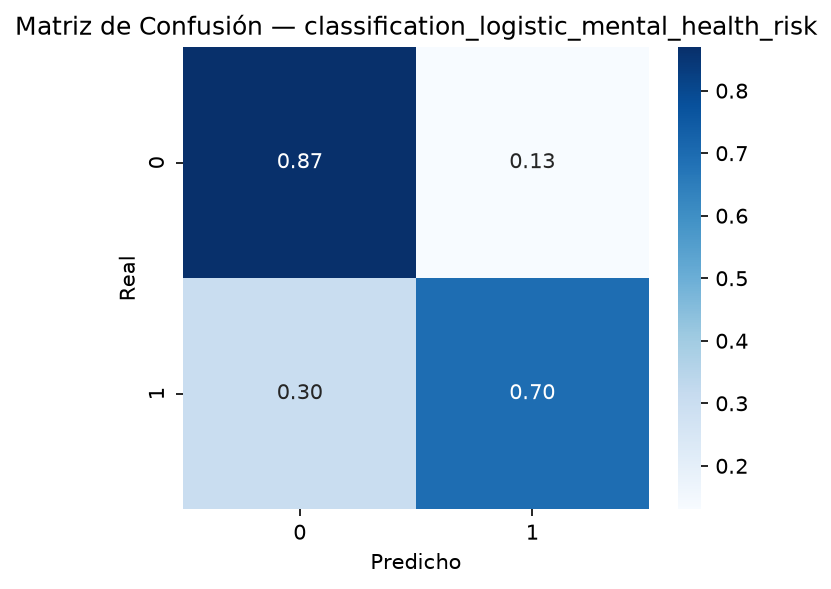
\includegraphics[width=0.85\columnwidth]{confusion_matrix_classification_logistic_mental_health_risk.png}
\caption{Matriz de confusión normalizada — Regresión Logística (riesgo de salud mental).}
\label{fig:confusion}
\end{figure}

\begin{figure}[h]
\centering
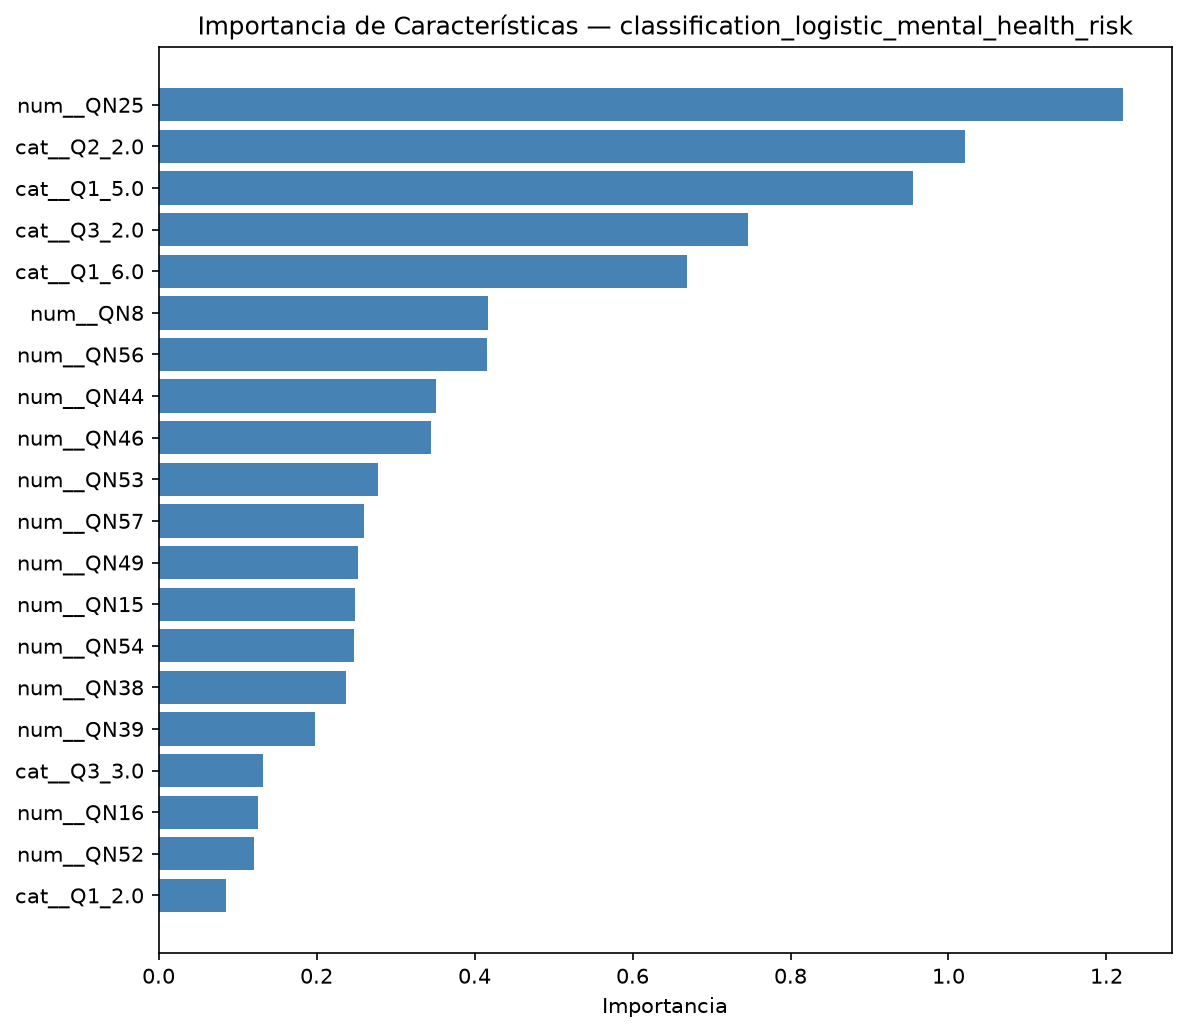
\includegraphics[width=0.85\columnwidth]{feature_importance_classification_logistic_mental_health_risk.png}
\caption{Importancia de características — Regresión Logística (riesgo de salud mental).}
\label{fig:importance}
\end{figure}

\subsection{Análisis de Ablación: ¿Qué Variables Importan?}

La Tabla~\ref{tab:ablation} presenta los resultados del análisis de ablación \textit{leave-one-group-out} partiendo de un F1 base de 0.491.

\begin{table}[h]
\caption{Análisis de ablación por grupos de variables (F1 clase en riesgo)}
\label{tab:ablation}
\centering
\begin{tabular}{@{}lcc@{}}
\toprule
\textbf{Grupo retirado} & \textbf{F1} & \boldmath{$\Delta$} \textbf{vs. base} \\
\midrule
(ninguno --- base)        & 0.491 & ---     \\
\textbf{Afectivo} (soledad, insomnio) & \textbf{0.437} & \boldmath{$-$0.054} \\
Consumo de sustancias     & 0.471 & $-$0.020 \\
Demografía (edad, sexo, grado) & 0.486 & $-$0.005 \\
Violencia / bullying      & 0.491 &  0.000  \\
Apoyo social              & 0.494 & $+$0.003 \\
Actividad física          & 0.500 & $+$0.008 \\
Dieta y nutrición         & 0.502 & $+$0.011 \\
\bottomrule
\end{tabular}
\end{table}

El resultado más claro: el grupo \textbf{afectivo} —que incluye la frecuencia con que el estudiante se siente solo y la presencia de insomnio por preocupación— es con diferencia el dominio más valioso. Su eliminación produce una caída de 0.054 puntos de F1, más del doble del impacto de cualquier otro grupo. El consumo de sustancias ocupa el segundo lugar ($\Delta = -0.020$). Sorprendentemente, retirar las variables de dieta, actividad física o apoyo social \textit{mejora} ligeramente el modelo, lo que sugiere que estos dominios aportan ruido en lugar de señal cuando el objetivo es predecir riesgo suicida.

% ============================================================
\section{Sistema Propuesto y Valor para la Política Pública}
% ============================================================

\subsection{Arquitectura del Sistema de Tamizaje}

El sistema propuesto opera en tres etapas:

\begin{enumerate}
  \item \textbf{Recolección}: encuesta escolar anual simplificada (15 preguntas clave del GSHS, priorizando los dominios afectivo y de consumo de sustancias) aplicada en centros educativos públicos.
  \item \textbf{Clasificación automatizada}: el pipeline entrenado clasifica a cada estudiante como ``en riesgo'' o ``sin riesgo detectado'' y genera reportes agregados por departamento y municipio.
  \item \textbf{Derivación}: los estudiantes clasificados como en riesgo son derivados a un protocolo de evaluación por personal de salud mental, no tratados directamente por el modelo.
\end{enumerate}

Este diseño respeta un principio fundamental: \textbf{el modelo es una herramienta de priorización poblacional, no un sustituto del diagnóstico clínico}. Su valor reside en identificar qué grupos y regiones requieren mayor atención, no en diagnosticar a individuos.

\subsection{Capacidad de Detección a Escala}

Con un AUC-ROC de 0.79, el clasificador logra una separación significativamente mejor que el azar (0.50). A modo ilustrativo: si El Salvador tiene aproximadamente 350,000 estudiantes en centros públicos de bachillerato, y la prevalencia de suicidalidad en la muestra GSHS es de $\approx$17\%, el modelo permitiría enfocar los recursos de tamizaje especializado en el subconjunto de mayor riesgo predicho, reduciendo la carga de evaluación clínica completa mientras aumenta la cobertura efectiva.

% ============================================================
\section{Limitaciones}
% ============================================================

Las siguientes limitaciones deben ser consideradas antes de implementar el sistema:

\begin{itemize}
  \item \textbf{Antigüedad de los datos}: el dataset data de 2013. Doce años de cambios socioeconómicos, pandemia y transformaciones en el uso de redes sociales pueden haber alterado los patrones de riesgo. La actualización mediante una nueva ronda GSHS es la recomendación más urgente.
  \item \textbf{Sesgo de autorreporte}: los adolescentes pueden subinformar comportamientos estigmatizados (consumo de sustancias, ideación suicida) o sobreinformar comportamientos deseables (actividad física). Este sesgo afecta directamente a los modelos entrenados sobre estos datos \cite{fisher1993social}.
  \item \textbf{Cobertura}: la muestra GSHS es escolar. Los adolescentes fuera del sistema educativo —frecuentemente los más vulnerables— no están representados.
  \item \textbf{Modelo de IMC inutilizable}: con $R^2 \approx 0$, el componente de regresión del IMC no debe emplearse para ninguna decisión clínica o de política.
  \item \textbf{Tasa de falsos negativos del clasificador}: un F1 de 0.558 implica que aproximadamente el 44\% de los estudiantes en riesgo no son detectados. Esta tasa es inaceptable para uso clínico individual, pero puede ser aceptable en un sistema de vigilancia poblacional donde el objetivo es reducir la brecha de atención, no garantizar cobertura perfecta.
\end{itemize}

% ============================================================
\section{Conclusiones y Recomendaciones}
% ============================================================

Este trabajo presenta evidencia empírica sobre los principales factores predictores de riesgo en adolescentes salvadoreños a partir del GSHS 2013. Los hallazgos más relevantes para la toma de decisiones en salud pública son:

\begin{enumerate}
  \item \textbf{Los síntomas afectivos son la señal más potente}: sentirse solo con frecuencia y presentar insomnio por preocupación predicen riesgo suicida con mayor fuerza que cualquier otro dominio medido. Las intervenciones que fortalezcan la salud emocional y los vínculos sociales tienen el mayor potencial de impacto.
  \item \textbf{El consumo de sustancias es el segundo factor modificable clave}: alcohol y drogas aparecen como co-predictores significativos. Los programas de prevención del uso de sustancias en escuelas tienen justificación empírica en esta muestra.
  \item \textbf{El IMC no es predecible desde encuestas conductuales}: invertir en programas de nutrición basados exclusivamente en autorreporte de comportamientos sería insuficiente; se requieren mediciones antropométricas directas en las escuelas.
  \item \textbf{La actualización de datos es la prioridad máxima}: ningún modelo entrenado sobre datos de 2013 puede sustituir una nueva ronda de encuesta GSHS. Se recomienda al Ministerio de Salud gestionar con la OMS la realización de un nuevo GSHS para El Salvador.
  \item \textbf{El sistema propuesto puede operar como herramienta de vigilancia epidemiológica}: el clasificador de salud mental (AUC-ROC = 0.79) tiene capacidad suficiente para priorizar grupos de riesgo a escala departamental si se integra en una encuesta escolar anual.
\end{enumerate}

\begin{thebibliography}{1}

\bibitem{who_gshs_2013}
World Health Organization, ``El Salvador --- Global School-based Student Health Survey 2013,'' WHO NCD Microdata Repository. [Online]. Available: \url{https://extranet.who.int/ncdsmicrodata/index.php/catalog/97}. [Accessed: Jun. 2026].

\bibitem{pedregosa2011scikit}
F. Pedregosa \textit{et al.}, ``Scikit-learn: Machine Learning in Python,'' \textit{Journal of Machine Learning Research}, vol. 12, pp. 2825--2830, 2011.

\bibitem{lemaitre2017imbalanced}
G. Lema\^{i}tre, F. Nogueira, and C. K. Aridas, ``Imbalanced-learn: A Python Toolbox to Tackle the Curse of Imbalanced Datasets in Machine Learning,'' \textit{Journal of Machine Learning Research}, vol. 18, no. 17, pp. 1--5, 2017.

\bibitem{breiman2001random}
L. Breiman, ``Random Forests,'' \textit{Machine Learning}, vol. 45, no. 1, pp. 5--32, 2001.

\bibitem{chawla2002smote}
N. V. Chawla, K. W. Bowyer, L. O. Hall, and W. P. Kegelmeyer, ``SMOTE: Synthetic Minority Over-sampling Technique,'' \textit{Journal of Artificial Intelligence Research}, vol. 16, pp. 321--357, 2002.

\bibitem{james2013introduction}
G. James, D. Witten, T. Hastie, and R. Tibshirani, \textit{An Introduction to Statistical Learning}, 1st ed. New York, NY, USA: Springer, 2013.

\bibitem{ieee754}
IEEE, ``IEEE Standard for Floating-Point Arithmetic,'' \textit{IEEE Std 754-2019}, pp. 1--84, 2019.

\bibitem{kaufman2012leakage}
S. Kaufman, S. Rosset, C. Perlich, and O. Stitelman, ``Leakage in Data Mining: Formulation, Detection, and Avoidance,'' \textit{ACM Transactions on Knowledge Discovery from Data}, vol. 6, no. 4, pp. 1--21, Dec. 2012.

\bibitem{patel2007mental}
V. Patel \textit{et al.}, ``Mental health of young people: a global public-health challenge,'' \textit{The Lancet}, vol. 369, no. 9569, pp. 1302--1313, Apr. 2007.

\bibitem{nock2008suicide}
M. K. Nock \textit{et al.}, ``Cross-national prevalence and risk factors for suicidal ideation, plans and attempts,'' \textit{The British Journal of Psychiatry}, vol. 192, no. 2, pp. 98--105, Feb. 2008.

\bibitem{davis2006relationship}
J. Davis and M. Goadrich, ``The relationship between Precision-Recall and ROC curves,'' in \textit{Proc. 23rd Int. Conf. Machine Learning (ICML)}, Pittsburgh, PA, USA, 2006, pp. 233--240.

\bibitem{fisher1993social}
R. J. Fisher, ``Social desirability bias and the validity of indirect questioning,'' \textit{Journal of Consumer Research}, vol. 20, no. 2, pp. 303--315, Sep. 1993.

\end{thebibliography}

\end{document}
